
\ifpdf
\graphicspath{{Chapter2/Chapter2Figs/PNG/}{Chapter2/Chapter2Figs/PDF/}{Chapter2/Chapter2Figs/}}
\else \graphicspath{{Chapter2/Chapter2Figs/EPS/}{Chapter2/Chapter2Figs/}} \fi

\chapter{Home network control scalability} 

In this chapter we explore the applications of SDN technologies in the home
network environment. Drawing conclusions from existing social and user studies,
we redesign the home network control abstraction. We present a Strawman
implementation of a network design which achieves simplicity and scalability of
the control abstraction within the home environment. Additionally, we propose an
extension of our design, which bridges the gap between the home network users
performance requirements and the ISP resource allocation policy, providing a
simple, scalable and user-friendly QoS mechanism.

In Section~\ref{s:elephant} we present a thorough review of ethnographic and
social studies and elaborate on the nature of the problems and the inherent
opportunities of the specific network environment. In Section~\ref{s:router}, we
describe our home router and how its flow-based approach enables it to help
improve the user experience. In section~\ref{s:protocols} we present and evaluate
protocol modifications that place the homeowner in more direct control of their
network. In section~\ref{s:qos} we present a simple QoS policy mechanism that
provides a communication channel between the home owner and the ISP and enables
a user friendly traffic scheduling mechanism for the ISP build using commodity
SDN applications. Finally, in Section~\ref{s:concl} we conclude the results of
our exploration.

Note that throughout this Chapter we refer to the individual managing the home
network as the homeowner without loss of generality; clearly any suitably
permitted member of the household, owner or not, may be able to exercise control
based on specifics of the local context. 

% \begin{itemize}
% \item We elaborate on the nature of the problems and opportunities inherent to
%       home networks~(\S\ref{s:elephant});
% \item We describe our home router and how its flow-based approach enables it to
%       help improve the user experience~(\S\ref{s:router}); and
% \item We present and evaluate protocol modifications that place the homeowner in
%       more direct control of their network~(\S\ref{s:protocols}).  
% \end{itemize}

%\mort{explicitly note we do not present user study but tech/infra dev deriving
%from ethno - user study is following in other papers}

% Finally, we present related work~(\S\ref{s:related}) and
% conclude~(\S\ref{s:concl}).  

\section{Technological and Social aspects of home networking} \label{s:elephant}

Consumer broadband Internet access is a critical component of the digital
revolution in domestic settings: for example, Finland has made broadband access
a legal right for all its
citizens~\footnote{\url{http://www.bbc.co.uk/news/10461048}}. A growing number
of services are now provided over the Internet, including government,
entertainment, communications, retail and health.  The growth of IP enabled
devices over the last decade also means many households are now exploring the
use of in-home wired and wireless networking, not only to allow multiple
computers to share an Internet connection but also to enable local media
sharing, gaming, and other applications.  In computer network literature, a
number of studies have been published that highlight the distinct properties of
the home network environment. In Subsection~\ref{s:home_measurement} we present
briefly the connectivity and traffic mix characteristics of home networks
based on the outcome of relevant studies, while in Subsection~\ref{s:home_social}
we discuss the relation of home networking technologies with the social context 
of the home, based on relevant ethnographic studies. 

% Despite the growth in Internet use and
% the explosion of interest in home networking, the opacity of networking
% technologies means that they remain extraordinarily difficult for people to
% install, manage, and use in their homes.

% {\it ``The technical know-how required to set up a network and run music or
%   video across cables or wi-fi, is `the elephant in the room that no-one wants
%   to talk
%   about.'\,''}\,\footnote{\url{http://news.bbc.co.uk/1/hi/technology/6949607.stm}}

\subsection{Home Networking as a system}

Home networks are highly heterogeneous edge networks, typically
Internet-connected via a single broadband link, where non-expert network
operators provide a wide range of services to a small set of users.  Internet
connectivity is through ADSL or cable connection, while there are also other
less popular links types found across the work, like fiber, 3g, satelite etc.
While we focus on home networks, we note that many environments, e.g.,~small
offices, coffee shops, hotels, exhibit similar characteristics and thus may
benefit from similar approaches. Such capabilities are likely to be infeasible
in more traditional settings, e.g.,~backbone and enterprise networks. 

Home network measurement studies have focused both on the local network
properties as well as the nature of the Internet traffic. Local network analysis
provides useful insight on the way devices interact within the house and the
possible performance limitations. Such measurement studies focused mainly on
developing active or passive measurement tools, that runs on end-hosts in the
network and collect data. In~\cite{homenetProfiler} authors develop an end-host
active  measurement tool accompanied by a small user survey, named HomeNet
Profiler. The analysis of the data unveils some interesting insights on home
network topology and connectivity. In terms of the size of home networks, users
report that their network consists on average of 7-8 device, but during the
measurement on average only 1-2 device were active in the network. Further, the
user survey reports a wide range of connected devices (e.g.  smartphones,
tablets, game consoles, etc.), which require from any designed solution to be as
much as possible open to device heterogeneity. Finally, the study also reports
useful statistics on wireless connectivity of end-hosts.  The study reports that
wifi connectivity to the home router is on average pretty good (signal strength
< -80dBm), but the medium appears to be over subscribed, with on average 10
active ssid discovered from the end-host wifi adapter during the measurement.
Further approximately 1/3 of the wireless networks exhibit channel overlap with
neighbouring networks. Interestingly, these observations point out the evolution
of wireless technology and contrast earlier results
on~\cite{Yarvis05characterizationof}. In terms of traffic mix,
in~\cite{Reggani12} authors analyse network traffic from a set of hosts in order
to understand how users use network applications in different environments. In
the home network environment, users tend to have distinct traffic mix.
Specifically, network filesystem and P2P applications generate significant
traffic volumes in the home environment, while a large portion of the traffic
remains local and can only be observed from within the network. 

Netalyzer~\cite{Kreibich20}, a web based java-applet that tests network
connectivity and protocol openness, provides useful insight on home networking.
Analysis of collected data unveiled a significant number of protocol
misconfiguration and malbehaving middleboxes in ISP networks. Additionally,
using a simple buffer flooding technique, the authors detect large packet buffer
in commercial home routers that can increase network latency up to 200 msec.
Additionally, in~\cite{Hatonen10} authors test a number of off-the-self home
router kit and discover that router firmwares exhibit a wide range of behaviours
in terms of NAT functionality and DNSEC support. Nontheless, because of the
popular usage of such routing kit, the impact to home networking appears to be
minimal and home network environment appears to be resilient to non-standard
router implementations. 

In terms of Internet connectivity, a number of studies have tried to analyse
residential networks in order to understand the properties of the traffic and
the impact of the ISP policies. Such analysis is also important at a
governmental level, in order to asses the quality of the ISP product and the
satisfiability of the clients~\ref{fcc, ofcomm}. Analysis of home network link
properties relies to a great extend  on BRAS level packet traces, or active
measurement probes from specific monitoring points. One of the first analysis on
this scope can be found in~\ref{Dischinger2007}, where an active measurement was
contacted in order to understand the properties of the link in residential
networks. The results of the analysis highlighted the important performance
differences between ISPs. The analysis pointed out that the bottleneck of the
end-to-end path for such networks was detected on the last mile of the link,
between the users modem and the BRAS of the ISP, while ISPs performance is
highly variable over the day. In~\cite{Sundaresan2011} authors follow a
different approach in measuring the network link and integrate various
measurement mechanisms in the home router firmware. In their analysis they
unveil a number of interest differences in the performance of a number of hosts
and point out that the very idea of performance is not clear and measurable by a
single test, while critical performance factors are distributed in various
points in the network.  

In terms of home network Internet traffic mix, research has highlighted highly
variable and location-dependent trends. In~\cite{Cho2006} authors describe that
during the time of their analysis in Japan there was a significant usage of P2P
applications. More recent studies~\cite{Maier2009} point out that users in
Germany have shifted interest towards web applications and a large portion of
the traffic in their trace was HTTP-based. Similar results are pointed out
in~\cite{Erman2011}, where http traffic is analysed into application types, and
online video and one-click hosting services appear as the predominant
application classes. 

\subsection{Home Network as a social activity}

Home networking technologies have been an interesting domain of study and
application for HCI, Ubiquitous computing and sociology, since it
provides an excellent environment to study the interaction between users and
technology. Studies in the fields usually engage in user interviews in order to
understand how users perceive and interact with technology. 

An important aspect in this is understanding how people perceive home network
technologies.
In~\cite{shehanpoole08:_desig_inter_home_networ_maint_tools,grinter05:_work_make_home_networ_work}
the authors ask from home network users to sketch their understanding of the
home network. In the sketch analysis the authors highlight two important
observations; user opacity to the network increases inversely proportional to
their network experience -- establishing  the effectiveness of the deep
abstraction-based design of the current network stack, and users characterize
network devices within the context of the home network. Further,
in~\cite{tolmie07:_makin} the authors perform an empirical analysis of the house
members with respect to technology and the home network.  Interestingly, their
finding detect that on average users are least motivated to interact with the
home network in order to optimize it as long as the perceived performance is
tolerable. Additionally, network maintenance is acceptable if it can resemble in
format the other household duties (well defined and simple tasks with short
durations), while the interest conflict that arise due to the shared nature of
some infrastructure is usually solved through negotiation between the household
members. An interesting study on this field is presented in~\cite{Chetty10}. In
this study, the authors develop a visualization system that inform home network
users with statistics on the network bandwidth usage. Interestingly, the
introduction of such a mechanism made users informed on the way the network
functions and how connectivity problems can be traced to network problem or to
other users.  Nontheless, such a technology also hinders the danger for users to
expose personal informations. 

A number of user studies have augmented the factors that shape home networking
adding as an important factor the design of the building within which the
network is installed. In~\cite{Rodden2003} authors describe a 7-layers model
devised by the American writer Stewart Brand in~\cite{Brand:1994} which
describes how homes evolve architecturally after their initial establishment.
Using this model authors analyse the relationships between Ubquitous
technologies and home design. This study is further focused on the home
networking technologies in~\cite{chetty07:_how_smart_homes_learn}. Authors
xontact a user study in order to understand how the home design relates to the
choices of users regarding their home network. The study describes how the user
network decisions are affected by the design of the house e.g. location of the
network router, while at the same time how the users confuse the limits of the
house with the limits of their network, e.g. users assume that encrypting their
home network is not important since it is contained within the limits of the
house.  In~\cite{rodden04:_between,crabtree03:_findin_place_ubicom_home} the
authors study a number of family homes and monitor the real time communications
and the ways in which information is produced and consumer within the house. In
their study they concluide that a lot of these activities have a location
reference within the house, which is related to the involved member as well as
the house planning, while activities can be synthesized as sequences into higher
order activities. Additionally, using these observations, they propose a
framework which can model such interactions. 

Finally, in~\cite{shehan07:_home_networ_hci} authors analyze some common
management and configuration problem in home networks and project them in the
respective design decisions of the network systems.  They present a weight of
evidence that problems with home networking are not amenable to solution via a
`thin veneer' of user interface technology layered atop the existing
architecture.  Rather, they are \emph{structural}, emerging from the mismatch
between the stable `end-to-end' nature of the Internet and the highly dynamic
and evolving nature of domestic environments.  

% Many empirical studies in recent years have explored the clear mismatch between
% current networking technology and the needs of the domestic setting,  in both
% the
% UK~\cite{}
% and the
% US~\cite{sung07:_my_roomb_rambo,}.
% These studies present a weight of evidence that problems with home networking
% are not amenable to solution via a `thin veneer' of user interface technology
% layered atop the existing architecture.  Rather, they are \emph{structural},
% emerging from the mismatch between the stable `end-to-end' nature of the
% Internet and the highly dynamic and evolving nature of domestic environments.  


\section{Motivations}\label{s:evolution}

\subsection{Home Network: Use cases}

Home networks use the same protocols, architectures, and tools developed for the
Internet since the 1970s.  Inherent to the Internet's `end-to-end' architecture
is the notion that the core is simple and stable, providing only a semantically
neutral transport service.  Its core protocols were designed for a certain
context of \emph{use} (assuming relatively trustworthy endpoints), made
assumptions about \emph{users} (skilled network and systems administrators both
using connected hosts and running the network core), and tried to accomplish a
set of \emph{goals} (e.g.,~scalability to millions of nodes) that simply do not
apply in a home network. 

In fact, the home network is quite different in nature to both core and
enterprise networks.  Existing
studies~\cite{tolmie07:_makin,shehan07:_home_networ_hci,shehanpoole08:_desig_inter_home_networ_maint_tools}
suggest domestic networks tend to be relatively small in size with between 5 and
20 devices connected at a time.  The infrastructure is predominately
cooperatively self-managed by residents who are seldom expert in networking
technology and, as this is not a professional activity, rarely motivated to
become expert.  A wide range of devices connect to the home network, including
desktop PCs, games consoles, and a variety of mobile devices ranging from
smartphones to digital cameras.  Not only do these devices vary in capability,
they are often owned and controlled by different household members.  

To illustrate the situation we are addressing, consider the following three
example scenarios, drawn from  situations that emerged from fieldwork 
reported in more detail elsewhere~\cite{wmust2011,chetty10}: 
 
\textbf{Negotiating acceptable use}.  {\it William and Mary have a spare room
  which they let to a lodger, Roberto.  They are not heavy network users and so,
  although they have a wireless network installed, they pay only for the lowest
  tier of service and they allow Roberto to make use of it.  The lowest tier of
  service comes under an acceptable use policy that applies a monthly bandwidth
  cap.  Since Roberto arrived from Chile they have exceeded their monthly cap on
  several occasions, causing them some inconvenience.  They presume it is
  Roberto's network use causing this, but are unsure and do not want to cause
  offence by accusing him without evidence.}

\textbf{Welcome visitors, unwelcome laptops}.  {\it Steve visits his friends
  Mike and Elisabeth for the weekend and brings his laptop and smartphone.  Mike
  has installed several wireless access points throughout his home and has
  secured the network using MAC address filtering in addition to WPA2.  To
  access the network, Steve must not only enter the WPA2 passphrase, but must
  also obtain the MAC addresses of his devices for Mike to enter on each
  wireless access point.  Steve apologizes for the trouble this would cause and,
  rather than be a problem to his hosts, suggests he reads his email at a local
  cafe.} 

\textbf{Sharing the medium socially efficient}.  {\it Richard is the teenage son
  of Derek and has a great interest in Music, downloading a lot of music from the
  Internet. Derek works some times in the night from home using the Terminal
  Services provided by his company. Tension is created between them as Derek
  blames Richard downloading activity for his poor performing remote desktop
  application. } 

In such ways, simple domestic activities have deep implications for
infrastructures that generate prohibitive technical overheads.  In the first
scenario, the problem is simply that the network's behaviour is opaque and
difficult for normal users to inspect; in the second, the problems arise from
the need to control access to the network and the technology details exposed by
current mechanisms for doing so.  

Home networks enable provision of a wide range of services, e.g.,~file stores,
printers, shared Internet access, music distribution.  The broad range of
supported activities, often blending work and leisure, make network use very
fluid.  In turn, this makes it very hard to express explicitly \emph{a priori}
policies governing access control or resource management~\cite{tolmie07:_makin}.
Indeed, fluidity of use is such that access control and policy may not even be
consistent, as network management is contingent on the household's immediate
needs and routines.

\subsection{Home Networks: Revolution!} \label{s:revolution}

Simply creating a user interface layer for the existing network infrastructure
will only reify existing problems.  Rather, we need to investigate creation of
new network architectures reflecting the socio-technical nature of the home by
taking into account both human and technical considerations. Control of the
network can be redefined, exposing only the required control and semantically
appropriate abstraction, in order to scale controllability of the network.  
% For example, we
% may need to explore architectures that sacrifice scalability in favor of
% installability, evolvability, and maintainability.  

To this end we exploit local characteristics of the home: devices are often
collocated, are owned by family and friends who physically bring them into the
home, and both devices and infrastructure are physically accessible.
Essentially, the home's physical setting provides a significant source of
heuristics we can understand, and offers a set of well understood practises that
might be exploited in managing the infrastructure.  

We exploit human understandings of the local network and the home to guide
management of the supporting
infrastructure~\cite{crabtree03:_findin_place_ubicom_home} by focusing on the
home router not only as the boundary point in an edge network but as a physical
device which can be exploited as a point of management for the domestic
infrastructure.  Within our router, we focus on flow management for three
reasons: \begin{itemize}
    \item we do not require forwarding scalability to the same degree as the core network; 
    \item doing so allows us to monitor traffic in a way that is more meaningful
      for users; and 
    \item we can apply per-flow queueing mechanisms to control bandwidth
      consumption, commonly requested by users.  \end{itemize}
%% \mort{distinction is now being pushed as: large-scale networks focus
%%      on packets not flows for scalability (plus other things of
%%      core/enterprise nets); we go for flows and explore impact of this
%%      decision} 

%% \mort{focusing on flows lets us (a) monitor traffic in a way that's
%%      (somewhat) meaningful for users (but cf.  wmust); (b) control
%%      traffic using a range of standard mechanisms such as per-flow
%%      queueing/qos} 

\section{Reinventing the Home Router} \label{s:router}
 
\begin{figure} 
  \centering 
  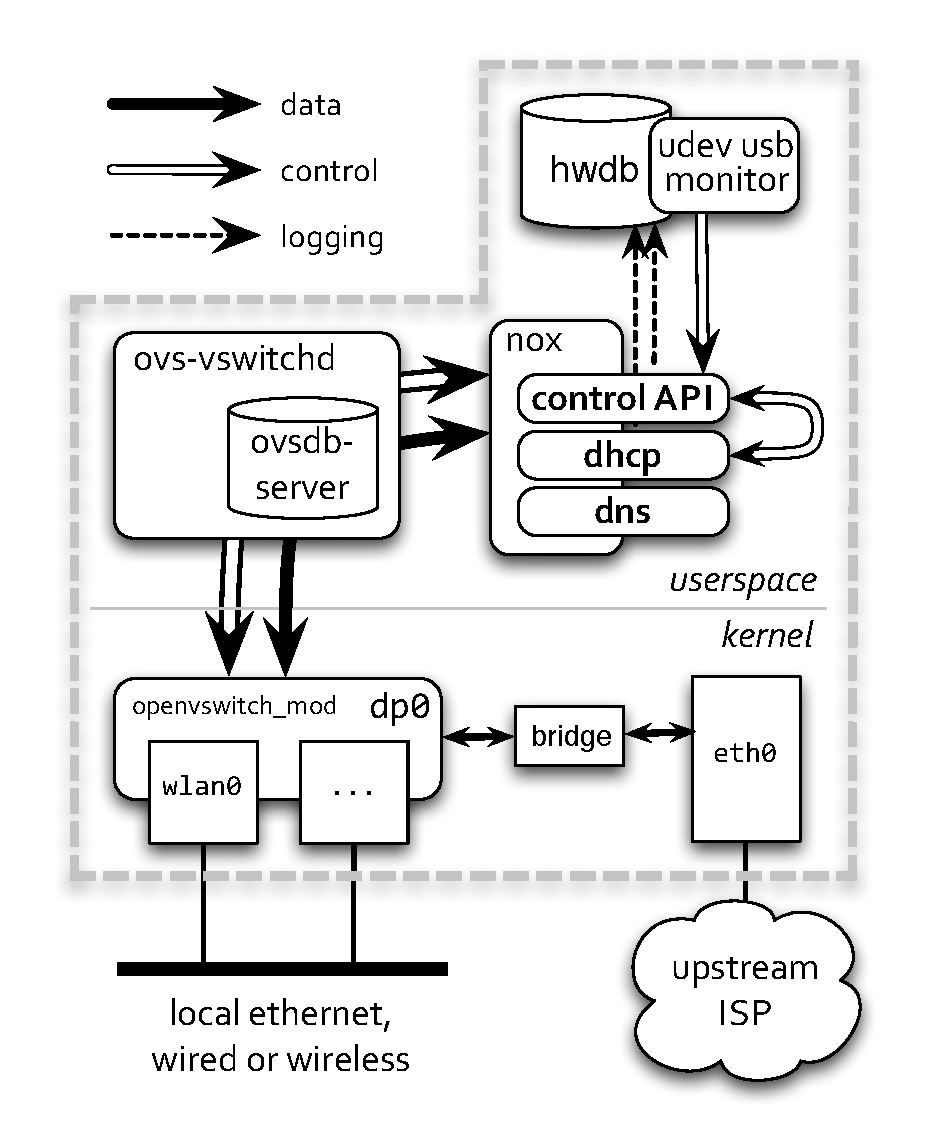
\includegraphics[trim=0.5cm 1cm 0.5cm 2.5cm, width=0.5\columnwidth]{architecture}
  \caption{\label{f:architecture}Home router architecture.  Open vSwitch
    (\emph{ovs*}) and NOX manage the wireless interface.  Three NOX modules
    provide a web services control API, a DHCP server with custom address
    allocation and lease management, and a DNS interceptor, all logging to the
    Homework Database (\emph{hwdb}) (\S\ref{s:protocols}). 
%% Finally, a udev script logs an
%% event to the Homework Database on USB stick insertion; a
%% subscribing process detects this and invokes the control API
%% appropriately (§5).} 
}\end{figure}

Our home router is based on Linux 2.6 running on a micro-PC
platform.\footnote{Currently an Atom 1.6GHz eeePC 1000H netbook with 2GB of RAM
  running Ubuntu 10.04.} Wireless access point functionality is provided by the
\emph{hostapd} package.  The software infrastructure on which we implement our
home router, as shown in Figure~\ref{f:architecture}, consists of the Open
vSwitch OpenFlow implementation, a NOX controller exporting a web service
interface to control custom modules that monitor and manage DHCP and DNS
traffic, plus the Homework
Database~\cite{sventek11:_infor_plane_archit_suppor_home_networ_manag} providing
an integrated network monitoring facility.
This gives us a setup very similar to a standard operator-provided home router
where a single box acts as wireless access point, multiplexes a wired
connection for upstream connectivity to the ISP, and may provide a small
number of other wired interfaces. 
  
%% \mort{static ip addresses?  still expect explicit configuration on
%%      router to enable connectivity- outside dhcp range; no big deal}

%% \mort{router runs hostapd, provides wireless ap with wpa2}

%% \mort{believed that some wireless cards may not permit access to all
%%      bridged packets- can we find a cite/link for this?} 
                                                                     
%% To allow us to explore how best to exploit the nature of the domestic
%% setting we need an infrastructure that can present information about
%% the nature of the activities on the network to users, and offers
%% capabilities to enable residents to control the network.  We have
%% built a home router based around Linux 2.6 on a micro-PC 
%% platform.\footnote{Currently an Atom 1.6GHz eeePC 1000H netbook with
%% 2GB of RAM running Ubuntu 10.04.} The software infrastructure on which
%% we implement our home router consists of a NOX controller using a set of custom modules
%% to control traffic and export a rich RPC API,
%% the Open vSwitch OpenFlow implementation, plus the Homework Database
%% providing an integrated network monitoring facility.\footnote{All our
%% code is publicly available; URL redacted for review.} Our home router
%% is implemented as an OpenFlow-enabled application, depicted in
%% Figure~\ref{f:architecture}.

 We next describe the main software components upon which our router relies.
  Using this infrastructure, we provide a number of novel user interfaces, one
  of which we describe briefly below; details of the others are available
  elsewhere~\cite{mortier11:_suppor_novel_home_networ_manag}.  Note that a key
  aspect of our approach is to avoid requiring installation of additional
  software on client devices: doing so is infeasible in a home context where so
  many different types of device remain in use over extended periods of time.

%% The router provides a platform to explore how the
%% infrastructure might change to provide better information to household
%% inhabitants, giving them greater understanding and control of their
%% home networks.  Before describing the details of our home router we
%% briefly present an overview of how these are presented to and
%% exploited by end-users.

\subsection{OpenFlow, Open vSwitch \& NOX} \label{s:openflow}

%% \mort{focus on flows makes openflow a natural control mechanism; plus
%%  it provides via ovs and NOX an efficient, straightforward and
%%  powerful programming api} 
 
% OpenFlow is a switching standard~\cite{mckeown:_openf} providing an open
% protocol for distributed control of the forwarding tables contained within
% Ethernet switches in a network.  An OpenFlow \emph{switch} has three parts: a
% \emph{datapath}, a \emph{secure channel} connecting to a controller, and the
% \emph{OpenFlow} \emph{protocol} the controller uses to talk to the switch.  
% 
% Each datapath applies actions to flows arising on a physical interface, where
% \emph{flow} is defined as a tuple of the primary packet header fields plus the
% physical port on which the flow is visible.  Flow definition allows wildcarding
% of fields and specifically permits netmasks for IP addresses.  Each flow can
% have a number of primitive actions applied; actions defined in the protocol
% permit full control over forwarding as well as modification of all fields of the
% flow tuple.  The net effect is that applications can manage and control traffic
% according to their own definition of a network flow.  Flow entries are installed
% by the controller when the switch notifies the controller of arrival of  a
% packet from a new flow.

We provide OpenFlow support using Open
vSwitch,\footnote{\url{http://openvswitch.org/}} OpenFlow-enabled switching
software that replaces the in-kernel Linux bridging functionality able to
operate as a standard Ethernet switch as well as providing full support for the
OpenFlow protocol.  We use the NOX\footnote{\url{http://noxrepo.org/}}
controller as it provides a programmable platform abstracting OpenFlow
interaction to events with associated callbacks, exporting APIs for C++ and
Python.

Our functionality is implemented in 5 different Nox modules.  C++ module {\it
  hwdb} synchronizes router state with the hwdb home
database~(Subsection~\ref{s:hwdb}), C++ module {\it
  homework\_dhcp} implements our custom DHCP server described later in
Section~\ref{s:protocol}, C++ module {\it homework\_routing} implements the
forwarding logic of the design, C++ module {\it homework\_dns} implements the DNS
interception functionality and Python module {\it homework\_rpc} exposes the
control API as a Web service. 

%% Currently, a set of libraries and applications
%% are implemented over the platform and exercise enriched control over
%% the network \haris{Maye provide some references to related work?}.

% The switching functionality is split between user and kernel space, for
% enhanced performance. In kernel space the Open vSwitch module stores a subset
% of exact match flows of the flow table, which is used as a flow cache, and
% implements all packet action primitives. The control plane of the switch is
% implemented on \emph{ovs-vswitchd}, a user space daemon. The daemon implements
% basic switch functionality, but is also able to communicate with OpenFlow
% controllers. Furthermore,  the daemon stores the complete Flow table of the
% switch as well as datapath configurations and translate them to appropriate
% data structures for the kernel module.

\begin{table}
  \begin{tabular} {p{0.35\columnwidth}p{0.55\columnwidth}} 
    \textbf{Method} & \textbf{Function} \\ 
    \url{permit/<eaddr>} & Permit access by specified client\\ 
    \url{deny/<eaddr>} & Deny access by specified client\\
    \url{status/[eaddr]} & Retrieve currently permitted clients, or status of specified client \\ 
    \url{dhcp-status/} & Retrieve current MAC--IP mappings\\
    \url{whitelist/<eaddr>} & Accept associations from client\\
    \url{blacklist/<eaddr>} & Deny association to client\\
    \url{blacklist-status/} & Retrieve currently blacklisted clients\\
    \url{permit-dns/<e>/<d>} & Permit access to domain \texttt{d} by client \texttt{e}\\ 
    \url{deny-dns/<e>/<d>} & Deny access to domain \texttt{d} by client \texttt{e}\\ 
  \end{tabular} 
  \caption{\label{t:api}Web service API;
    prefix all methods \texttt{https://.../ws.v1/}.  $<$\,$X$\,$>$ and $[X]$
    denote required and optional parameters.}
\end{table}

Our router provides flow-level control and management of traffic via a single
OpenFlow datapath managing the wireless interface of the
platform.\footnote{Without loss of generality, our home route has only a single
  wired interface so the only home-facing interface is its wireless interface;
  other home-facing interfaces would also become part of the OpenFlow datapath.}
We provide NOX modules that implement a custom DHCP server, control forwarding,
control wireless association via filtering, and intercept DNS lookups.  Control
of these modules is provided via a simple web service (Table~\ref{t:api}).
% within NOX whose interface is described in Table~\ref{t:api}.  
Traffic destined for the upstream connection is forwarded by the datapath for
local processing via the kernel bridge, with Linux's \emph{iptables} IP
Masquerading rules providing standard NAT functionality.\footnote{While NAT
  functionality could be implemented within NOX, it seemed neither interesting
  nor necessary to do so.}

%% Without loss of generality, the device we describe in this paper has
%% only a single wired interface so the only home facing interface is its
%% wireless interface, and this is the physical interface managed by the
%% OpenFlow datapath.

\subsection{The Homework Database} \label{s:hwdb}
 
%% \mort{reduce this- it's reported elsewhere: it's a streaming database,
%%  collecting ip layer supporting rpc interaction, and defaults to providing
%%  a Flows table among others; provides the basic measurement
%%  facility accessed by the many uis via rpc}
 
In addition to Open vSwitch and NOX we make use of the Homework Database,
\emph{hwdb}, an active, ephemeral stream
database~\cite{sventek11:_infor_plane_archit_suppor_home_networ_manag}.  The
ephemeral component consists of a fixed-size memory buffer into which arriving
tuples (events) are stored and linked into tables.  The memory buffer is treated
in a circular fashion, storing the most recently received events inserted by
applications measuring some aspect of the system.  The primary ordering of
events is time of occurrence.  

The database is queried via a variant of CQL~\cite{arasu05:_cql} able to express
both temporal and relational operations on data, allowing applications such as
our user interfaces to periodically query the ephemeral component for either raw
events or information derived from them. 
Applications need not be collocated on the router as \emph{hwdb} provides a
lightweight, UDP-based RPC system that supports one-outstanding-packet semantics
for each connection, fragmentation and reassembly of large buffers, optimization
of ACKs for rapid request/response exchanges, and maintains liveness for
long-running exchanges.  Monitoring applications request can execute temporal
query on specific types of events.  \emph{hwdb} also provides notification
functionality; applications may register interest in \emph{future} behaviour
patterns and receive notification when such patterns occur in the
database.  The work described in this paper makes use of three tables:
\emph{Flows}, accounting traffic to each 5-tuple flow; \emph{Links}, monitoring
link-layer performance; and \emph{Leases}, recording mappings assigned via DHCP.

%% By default, there are three tables, Flows, Links, and Leases.  Table
%% Flows stores the number of packets and bytes as observed (inserted) by
%% an application that accumulates these counts for each 5-tuple flow per
%% measurement interval (currently set to 1s in our deployments).  In a
%% similar manner, table Links stores the average RSSI, the number of
%% packets, the number of bytes, and the number of retransmissions
%% observed for each wireless device identified by its MAC
%% address.  Finally, table Leases stores any actions taken by the DHCP
%% server (e.g., granting or revoking a lease) with the mappings between
%% allocated IP addresses and host MAC addresses and names.  

%% \mort{fix link para}

%% We next describe details, implementation and evaluation of the two
%% strategies by which we exploit the home network context.  First we
%% consider the ways in which people may be more directly involved in
%% infrastructure protocols.


\subsection{The Guest Board} \label{s:guest-board}

% \mort{explicitly tie to ethno story} 

\begin{figure} 
  \centering 
  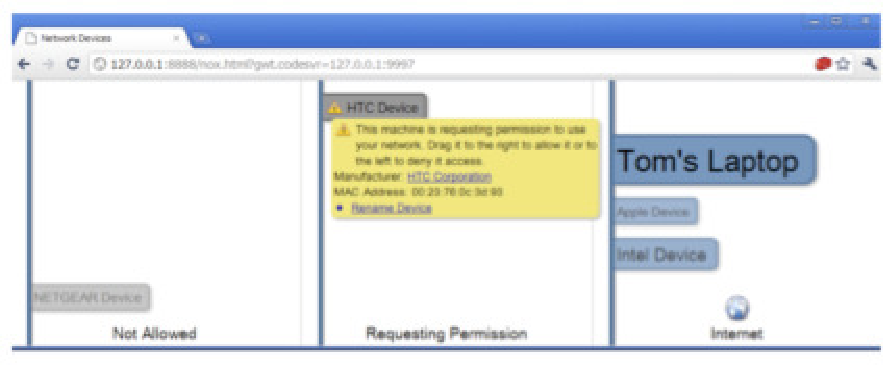
\includegraphics[width=0.5\columnwidth]{control-test}
  \caption{\label{f:guest-board}The \emph{Guest Board} control panel, showing an
    HTC device requesting connectivity.}
\end{figure}

This interface exploits people's everyday understanding of control panels in
their homes, e.g.,~heating or alarm panels, to provide users with a central
point of awareness and control for the network. We exploit this physical arrangement to
provide a focal point for inhabitants to view current network status and to
manage the network.  It provides a real time display of the current status of
the network (Figure~\ref{f:guest-board}), showing devices in different zones
based on the state of their connectivity.  The display dynamically maps key
network characteristics of devices to features of their corresponding labels.
Mappings in the current display are: 

\begin{itemize}
\item Wireless signal strength is mapped to device label transparency, so
      devices supplying weak signals fade into the background.
\item Device bandwidth use is proportional to its label size, e.g.,~Tom's Laptop
      in Figure~\ref{f:guest-board} is currently the dominant bandwidth user. 
\item Wireless Ethernet retransmissions show as red highlights on the device's
  label, indicating devices currently experiencing wireless reliability problems. 
\end{itemize}

Devices in range appear on the screen in real-time, initially in the leftmost
panel indicating they are within range of the home router but not connected.
The central panel in the control displays machines actively seeking to associate
to the access point. This zone exploits the underlying
strategy of placing people in the protocol discussed in~\S\ref{s:protocol}.  
When devices unknown to the network issue DHCP requests, the router's DHCP
server informs the guest board and a corresponding label appears in this portion
of the display.  If a user wishes to give permission for the machine to join the
network they drag the label to the right panel; to deny access, they drag the
label to the left panel.

The guest board provides both a central control point and, by drawing directly
upon network information collected within our router, a network-centric view of
the infrastructure.  The interface is implemented in HTML/CSS/Javascript
allowing it to be displayed on a range of devices, currently under trial with
users.  The router's measurement and control APIs described above are also being
used to build a wide range of other interfaces for use via smartphones, web
browsers, and custom display hardware.
%% \mort{...it is just one of several interfaces we have built that use
%%  the features of our home router, ranging from network artefacts
%%  to phyiscally mediated access via usb key tokens; see uist2011
%%  paper insub for details}

\section{Putting People in the Protocol} \label{s:protocols}

%\mort{note that this is tied to social convention of home visiting, network
%part of the home not separate to it, etc}
We use our home router to enable \emph{ad hoc} control of network policy by
non-expert users via interfaces such as the Guest Board
(Figure~\ref{f:guest-board}).  This sort of control mechanism is a natural fit
to the local negotiation over network access and use that takes place in most
home contexts.  While we believe that this approach may be applicable to other
protocols, e.g.,~NFS/SMB, LPD, in this section we demonstrate this approach via
our implementation of a custom DHCP server and selective filters for wireless
association and DNS that enable management of device connectivity on a
per-device basis. 

Specifically, we describe and evaluate how our router manages IP address
allocation via DHCP, two protocol-specific (EAPOL and DNS) interventions it
makes to provide finer-grained control over network use, and its forwarding
path.  We consider three primary axes: \emph{heterogeneity} (does it still
support a sufficiently rich mix of devices); \emph{performance} (what is the
impact on forwarding latency and throughput of our design and implementation
decisions); and \emph{scalability} (how many devices and flows can our router
handle).  In general we find that our home router has ample capacity to support
observed traffic mixes, and shows every indication of being able to scale beyond
the home context to other situations, e.g., small offices, hotels. 

\subsection{Address Management} \label{s:addresses}

DHCP~\cite{rfc:2131} is a protocol that enables automatic host network
configuration. It is based on a four way broadcast handshake that allows hosts
to discover and negotiate with a server their connectivity parameters.  As part
of our design we extend the functionality of the protocol to achieve two goals.
First, we enable the homeowner to control which devices are permitted to connect
to the home network by interjecting in the protocol exchange on a case-by-case
basis.  We achieve this by manipulating the lease expiry time, allocating only a
short lease (30s) until the homeowner has permitted the device to connect via a
suitable user interface.  The short leases ensure that clients will keep
retrying until a decision is made; once a device is permitted to connect, we
allocate a standard duration lease (1 hour).

Second, we ensure that all network traffic is visible to the home router and
thus can be managed through the various user interfaces built against it.  We do
so by allocating each device to its own /30 IP subnet, forcing inter-device
traffic to be IP routed via our home router.  This requirement arises because
wireless Ethernet is a broadcast medium so clients will ARP for destinations on
the same IP subnet enabling direct communication at the link-layer.  In such
situations, the router becomes a link-layer device that simply schedules the
medium and manages link-layer security -- some wireless interfaces do not even
make switched Ethernet frames available to the operating system. The result
is that traffic between devices in the
home, such as music distribution and file stores, becomes invisible to the
home router.  By allocating addresses from distinct subnets, all traffic
between clients must be transmitted to the gateway address, ensuring all
traffic remains visible to our home router. 
Our custom DHCP server allocates /30 subnet to each host from 10.2.*.*/16 with
standard address allocation within the /30 (i.e.,~considering the host part of
the subnet, 00 maps to the network, 11 maps to subnet broadcast, 01 maps to the
gateway and 10 maps to the client's interface itself). Thus, each local device
needs to route traffic to any other local device thought the router, making
traffic visible in the IP layer.
%% We deal with the case of
%% misbehaving/malicious clients attempting to subvert our address
%% allocations in~\S\ref{s:association}. 
% \mort{point to lack of perf implications?  or just pull to here?}
%
% The DHCPOFFER generated by our home router in response to a previously unknown
% client allocates a /30 subnet from 10.2.*.*/16 with standard address
% allocation within the /30 (i.e.,~considering the two least significant bits of
% the subnet, 00 maps to the network, 11 maps to subnet directed broadcast, 01
% maps to the gateway and 10 maps to the client's interface itself).  This
% allocation pattern ensures that all traffic for locally connected devices is
% sent via the router, since all devices are on distinct, non-overlapping IP
% subnets.  This would not be the case if addresses were allocated to clients
% from the same subnet, e.g.,~clients were all simply allocated addresses
% directly from 10.*.*.*/8.

We measured the performance of our DHCP implementation and found that, as
expected, per-request service latency scales linearly with the number of
simultaneous requests.  Testing in a fairly extreme scenario, simultaneous
arrival of 10 people each with 10 devices,  gives a median per-host service time
of 0.7s.

\subsection{Per-Protocol Intervention} \label{s:association}

Our current platform intervenes in two specific protocols providing greater
control over access to the wireless network itself, and to Internet services
more generally. 

\begin{figure} \centering 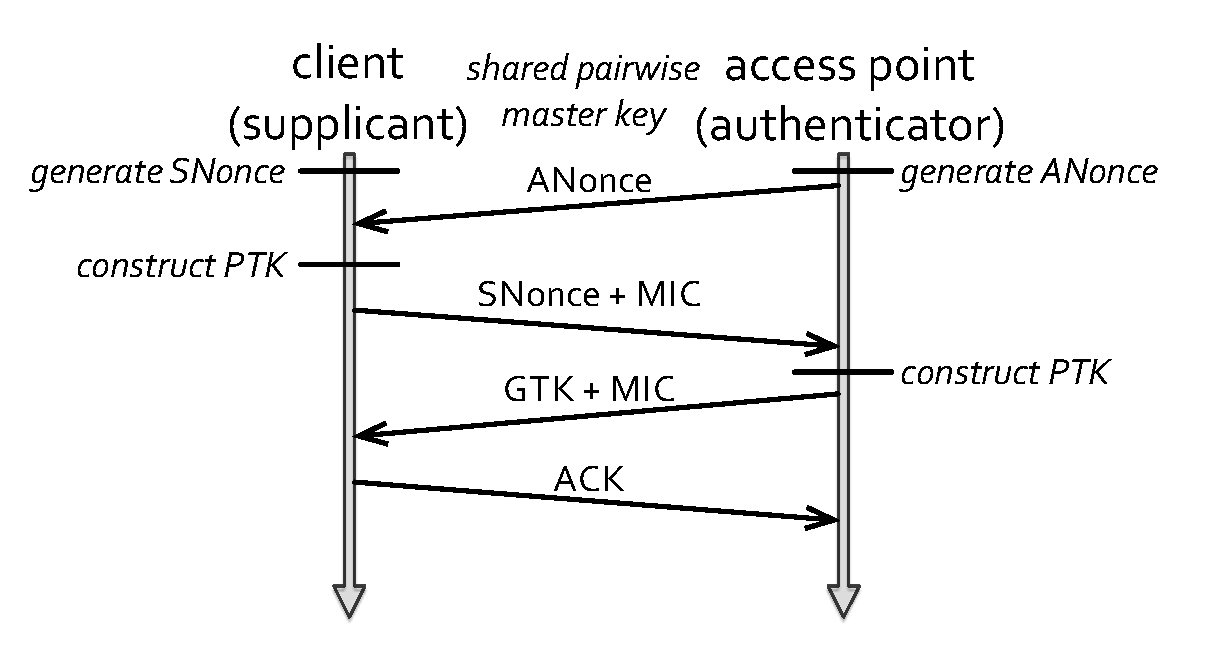
\includegraphics[width=0.8\columnwidth]{eapol}
  \caption{\label{f:association}802.11i handshake, part of the association
    process.  Note that MIC (Message Integrity Code) is an alternate term for
    MAC, used in such contexts to avoid confusion with Media Access Control.}
  \end{figure}
 
%% \mort{also intercept DNS- figures from previous section show that this
%%      will introduce negligible extra latency} 

Our home router supports wireless Ethernet security via 802.11i with EAP-WPA2,
depicted in Figure~\ref{f:association}, using \emph{hostapd}.  In short, the
client (\emph{supplicant}) and our router (\emph{authenticator}) negotiate two
keys derived from the shared master key via a four-way handshake, through the
EAPOL protocol.  The \emph{Pairwise Transient Key} (PTK) is used to secure and
authenticate communication between the client and the router; the \emph{Group
  Transient Key} (GTK) is used by the router to broadcast/multicast traffic to
all associated clients, and by the clients to decrypt that traffic.  All
non-broadcast communication between clients must therefore pass via the router
at the link-layer (for decryption with the source's PTK and re-encryption with
the destination's PTK), although the IP routing layers are oblivious to this if
the two clients are on the same IP subnet.\footnote{The 802.11i specification
  defines a general procedure whereby two clients negotiate a key for mutual
  communication (\emph{Station-to-station Transient Key}, STK).  However, the
  only use of this procedure in the specification is in \emph{Direct Link Setup}
  (DLS) used in supporting 802.11e, quality-of-service.  This can easily be
  blocked by the access point, and in fact is not implemented in the
  \emph{hostapd} code we use, so we do not consider it further.
  %\mort{emphasise this bit?  also wifidirect - embedding of ``soft'' ap inside
  %wifi device - completely orthogonal?}i
  }

Periodically, a timeout event at the access point initiates rekeying of the PTK,
visible to clients only as a momentary drop in performance rather than the
interface itself going down.  We use this to apply blacklisting of clients
deemed malicious, such as a client that attempts to communicate directly (at the
link-layer) with another, i.e.,~attempting to avoid their traffic being visible
to our home router.  We wait until the rekeying process begins and then decline
to install the appropriate rule to allow it to complete for the client in
question.  This denies the client access even to link-layer connectivity, as
they will simply revert to performing the four-way handshake required to obtain
the PTK.  This gives rise to a clear trade-off between security and performance:
the shorter the rekeying interval, the quicker we can evict a malicious client
but the greater the performance impact on compliant clients.  

\begin{figure} \centering 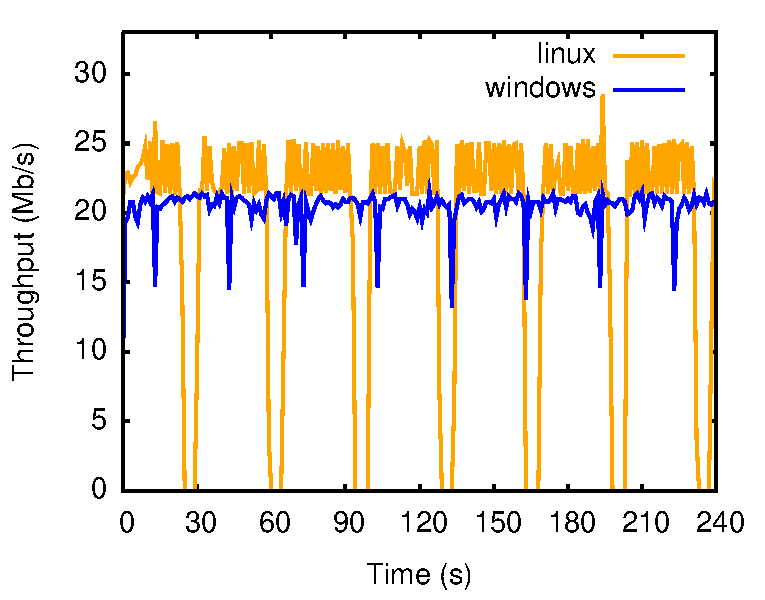
\includegraphics[width=0.7\columnwidth]{rekeying}
  \caption{\label{f:rekeying}Affect on TCP throughput from rekeying every 30s
    for Linux 2.6.35 using a Broadcom card with the \emph{athk9} module; and
    Windows 7 using a proprietary Intel driver and card.} 
\end{figure}

\begin{figure*} \centering
  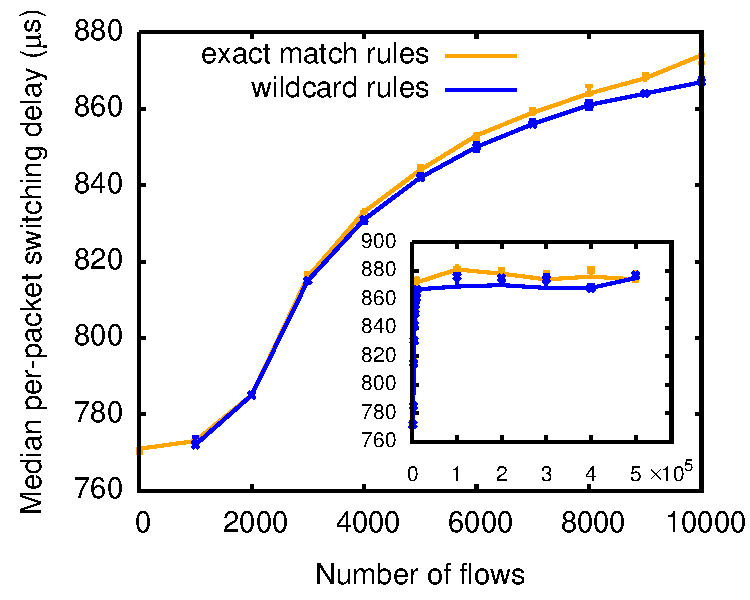
\includegraphics[width=0.49\columnwidth]{switching-delay}
  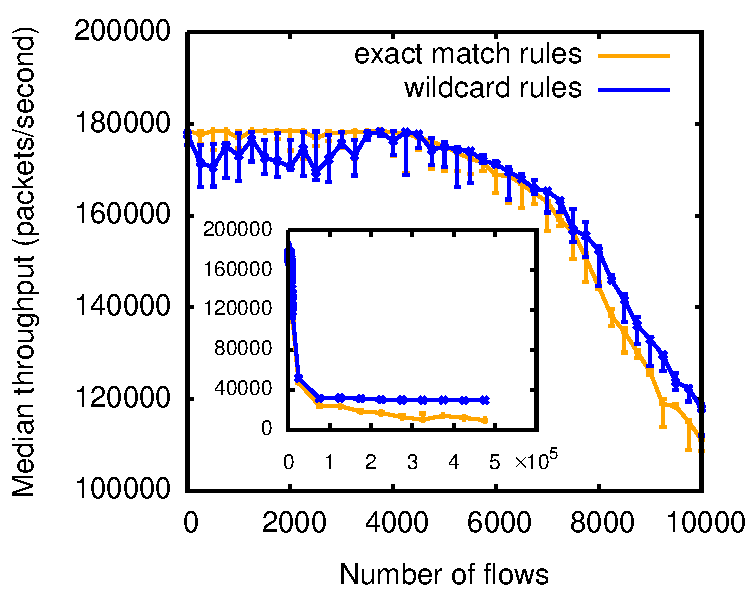
\includegraphics[width=0.49\columnwidth]{throughput}
  \caption{\label{f:performance}Switching performance of Open vSwitch component
    of our home router showing increasing per-packet latency (LHS) and
    decreasing packet throughput (RHS) with the number of flows.  The inset
    graph extends the $x$-axis from 10,000 to 500,000.}
\end{figure*}

To quantify the impact of 802.11i rekeying, we observed throughput over several
rekeying intervals.  Figure~\ref{f:rekeying} shows the impact of setting the
rekeying interval to 30s: rekeying causes a periodic dip in throughput as the
wireless Ethernet transparently buffers packets during rekeying before
transmitting them as if nothing had happened.  This shows the trade-off between
performance and responsiveness of this approach
: to be highly responsive in detection of misbehaving clients imposes a small
performance degradation.  
As a compromise, when a device is blacklisted, all of its traffic and subsequent
rekeying exchanges are blocked.
Thus the misbehaving device is prevented from sending or directly receiving any
traffic before rekeying takes place, 
The device will be able to receive only broadcast traffic in the interim due, to
the use of the GTK for such frames, until the AP initiate the negotiation of a
new key.  
This allows us to pick a relatively long rekey interval (5 minutes) while
still being able to respond quickly to misbehaving devices.

We also intercept DNS to give fine-grained control over access to Internet
services and websites.  DNS requests are intercepted and dropped if the
requesting device is not permitted to access that domain.  Any traffic the
router encounters that is not already permitted by an explicit OpenFlow flow
entry has a reverse lookup performed on its destination address.  If the
resulting name is from a domain that the source device is not permitted to
access, then a rule will be installed to drop related traffic.  Performance is
quite acceptable, as indicated by latency results in Figure~\ref{f:performance}:
the extra latency overhead introduced by our router is negligible compared to
the inherent latency of a lookup to a remote name server.  
% Extending this
% fine-grained control requires more accurate identification of traffic to
% application, particularly for more complex network uses such as BitTorrent and
% Skype, and is a problem we are investigating in ongoing work.

\subsection{Forwarding} \label{s:forwarding}
 
Our router consists of a single Open VSwitch that manages interface
\emph{wlan0}.  Open VSwitch is initialised with a set of flows that push
DHCP/BOOTP and IGMP traffic to the controller for processing.
OpenVSwitch by default will also forward to the controller traffic not matched
by any other installed flow, which is handled as follows:

\textbf{Non-IP traffic}.  The controller acts as a proxy ARP server, responding
to ARP requests from clients.  Misbehaving devices are blacklisted via a rule
that drops their EAPOL~\cite{rfc:3748} traffic thus preventing session keys
negotiation.
% implementing the WPA security association with the access point, so dropping
% it, prevents association.  
Finally, other non-IP non-broadcast traffic has source and destination MAC addresses verified
to ensure both are currently permitted.  If so, the packet is forwarded up the
stack if destined for the router, or to the destination otherwise.  In either
case, a suitable OpenFlow rule with a 30s idle timeout is also installed to
shortcut future matching traffic.

\textbf{Unicast IP traffic}.  First, a unicast packet is dropped if it does not
pass all the following tests: 
\begin{itemize}
    \item its source MAC address is permitted; 
    \item its source IP address is in 10.2.x.y/16; and
    \item its source IP address matches that allocated by DHCP.  For valid
      traffic destined to the Internet, a flow is inserted that forwards packets
      upstream via the bridge and IP masquerading.  
\end{itemize} 
Unicast IP traffic that passes but is destined outside the home network has a
rule installed to forward it upstream via the bridge and IP masquerading.  For
traffic that is to remain within the home network a flow is installed to route
traffic as an IP router, i.e.~rewriting source and destination MAC addresses
appropriately.  All these rules are installed with 30s idle timeouts, ensuring
that they are garbage collected if the flow goes idle for over 30s.

\textbf{Broadcast and multicast IP traffic}.  Due to our address allocation
policy, broadcast and multicast IP traffic requires special attention.  Clients
send such traffic with the Ethernet broadcast bit\footnote{I.e.,~the most
  significant bit of the destination address} set, normally causing the hardware
to encrypt with the GTK rather than the PTK so all associated devices can
receive and decrypt those frames directly.  In our case, if the destination IP
address is all-hosts broadcast, i.e.,~255.255.255.255, the receiver will process
the packet as normal.  Similarly, if the destination IP address is an IP
multicast address, i.e.,~drawn from 224.*.*.*/4, any host subscribed to that
multicast group will receive and process the packet as normal. Finally, for
local subnet broadcast the router will rebroadcast the packet, rewriting the
destination IP address to 255.255.255.255. This action is required because the
network stack of the hosts filters broadcast packets from different IP subnets.

To assess switching performance, we examine both latency and packet throughput
as we increase the number of flows, $N$, from 1--500,000.  Each test runs for
two minutes, generating packets at line rate from a single source to $N$
destinations each in its own 10.2.*.*/30 subnet.  As these are stress tests we
use large packets (500B) for the latency tests and minimal packets (70B)
\footnote{The 30B extra overhead is due to
  \emph{pktgen}~\cite{olsson05:_linux_packet_gener}, the traffic generation tool
  used.} for the throughput tests, selecting destinations at random on a
per-packet basis.  Results are presented as the median of 5 independent runs
with error bars giving the min and max values. 

Figure~\ref{f:performance} shows median per-packet switching delay and per-flow
packet throughput using either exact-match rules or a single wildcard rule per
host.  Performance is quite acceptable with a maximum switching delay of
560$\mu$s and minimum throughput of 40,000 packets/second; initial deployment
data suggests a working maximum of 3000 installed flows which would give around
160,000 packets/second throughput (small packets) and 500$\mu$s switching delay
(large packets).  Figure~\ref{f:stack-throughput} shows that the Linux
networking stack is quite capable of handling the unusual address allocation
pattern resulting from the allocation of each wireless-connected device to a
distinct subnet which requires the router's wireless interface to support an IP
address per connected device. 

\subsection{Discussion}

Our evaluation shows that OpenvSwitch can handle orders of magnitude more rules
than required by any reasonable home deployment.  Nonetheless, to protect
against possible denial-of-service attacks on the flow tables, whether
intentional, accidental or malicious, our home router monitors the number of
per-flow rules introduced for each host.  If this exceeds a high threshold then
the host has its per-flow rules replaced with a single per-host rule, while the
router simultaneously invokes user interfaces to inform the homeowner of the
device's odd behaviour. 

The final aspect to our evaluation is compatibility: given that our router
exercises protocols in somewhat unorthodox ways, how compatible is it with
standard devices and other protocols?  We consider compatibility along three
separate dimensions: range of existing client devices; deployed protocols that
rely on broadcast/multicast behaviours; and support for IPv6. 

\begin{figure} \centering 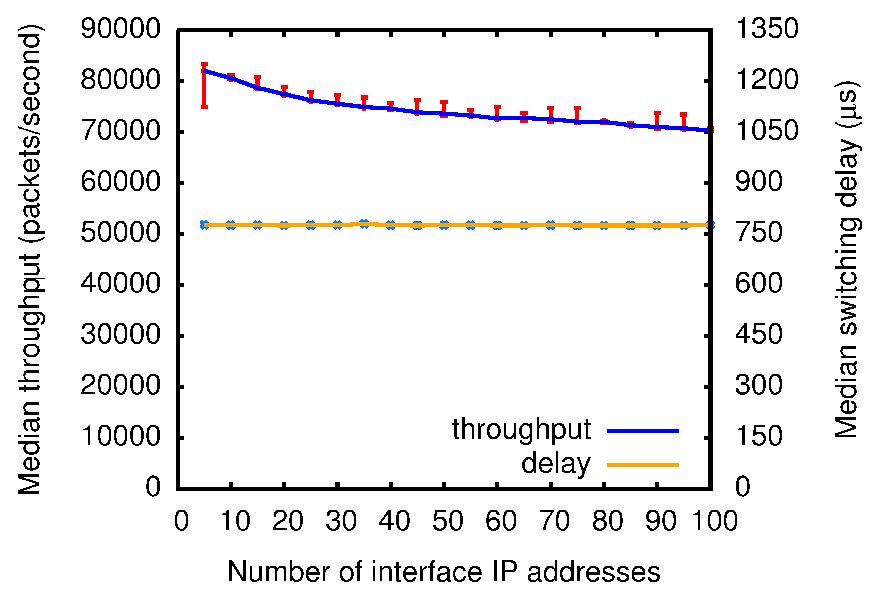
\includegraphics[width=\columnwidth]{stack-throughput}
  \caption{\label{f:stack-throughput}Switching performance of Linux network
    stack under our address allocation policy. Throughput (left axis) shows a
    small linear decrease while switching delay (right axis) remains
    approximately constant as the number of addresses allocated to the interface
    increases.} \end{figure}

\paragraph{Devices} Although we exercise DHCP, DNS and EAPOL in unorthodox ways
to control network access, behaviour follows the standards once a device is
permitted access.  To verify that our home router is indeed suitable for use in
the home, we tested against a range of commercial wireless devices running a
selection of operating systems. 

\begin{table*} \centering\footnotesize
  \begin{tabular}{lp{0.33\textwidth}p{0.42\textwidth}} \bf Device & \bf Denied &
    \bf Blacklisted\\

Android 2.x & Reports pages unavailable due to DNS.  & Retries several times
before backing off to the 3g data network.\\

iTouch/iPhone & Reports server not responding after delay based on configured
DNS resolver timeout.  & Requests new wireless password after 1--2 minutes.\\

OSX 10.6 & Reports page not found based on configured DNS resolver timeout.  &
Requests new wireless password after 1--2 minutes.\\

Microsoft Windows XP & Silently fails due to DNS failure.  & Silently
disconnects from network after 4--5 minutes.\\

Microsoft Windows 7 & Warns of partial connectivity.  & Silently disconnects
from network after 4--5 minutes.\\

Logitech Squeezebox & Reports unable to connect; allows server selection once
permitted.  & Flashes connection icon every minute as it attempts and fails to
reconnect.  \\ 

Nintendo Wii & Reports unable to reach server during ``test'' phase of
connection.  & Reports a network problem within 30s.\\

Nokia Symbian OS & Reports ``can't access gateway'' on web access.  & Reports
disconnected on first web access.\\ \end{tabular}
\caption{\label{t:devices}Observed interactions between devices and our home
  router when attempting to access the network.}
\end{table*}

Table~\ref{t:devices} shows the observed behaviour of a number of common
home-networked devices: in short, all devices operated as expected once
permitted access.  DNS interception was not explicitly tested since, as an
inherently unreliable protocol, all networking stacks must handle the case that
a lookup fails anyway.  Most devices behaved acceptably when denied access via
DHCP or EAPOL, although some user interface improvements could be made if the
device were aware of the registration process.  The social context of the home
network means no problem was serious: in practice the user requesting access
would be able to interact with the homeowner, enabling social negotiation to
override any user interface confusion. 

%% We initially investigated using different subnet allocations with
%% short (30s) lease times to more easily distinguish hosts that are
%% trying to connect but are waiting for the homeowner to permit them
%% access.  Unfortunately, due to a variety of issues with common client
%% DHCP implementations, e.g., Android not correctly obeying lease
%% times,\footnote{\url{http://www.net.princeton.edu/android/android-stops-renewing-lease-keeps-using-IP-address-11236.html}} 
%% this broke device interfaces sufficiently that doing so would only
%% increase user confusion.

\paragraph{Broadcast protocols} A widely deployed set of protocols relying on
broadcast and multicast behaviours are those for `zero conf' functionality.  The
most popular are Apple's \emph{Bonjour} protocol; \emph{Avahi}, a Linux variant
of Bonjour; Microsoft's \emph{SSDP} protocol, now adopted by the UPnP forum; and
Microsoft's \emph{NetBIOS}.  

Bonjour and Avahi both rely on periodic transmission of multicast DNS replies
advertising device capabilities via TXT records.  SSDP is similar, but built
around multicast HTTP requests and responses.  We tested Bonjour specifically by
setting up a Linux server using a Bonjour-enabled daemon to share files.  We
observed no problems with any clients discovering and accessing the server, so
we conclude that Bonjour, Avahi and SSDP would all function as expected. 

NetBIOS is somewhat different, using periodic network broadcasts to disseminate
hosts' capabilities.  In doing so we observed a known deficiency of NetBIOS: it
cannot propagate information for a given workgroup between different
subnets.\footnote{\url{http://technet.microsoft.com/en-gb/library/bb726989.aspx}}
However this was easy to overcome: simply install a WINS server on the router
and advertise it via DHCP to all hosts.
%\mort{although ugly, this would work at little cost and the other benefits seem
%significant. no extra attack surface because can configure nox/ovs/firewall to
%deny access to it from outside the home network}

In general, it may seem that our address allocation policy introduces link-layer
overhead by forcing all packets to be transmitted twice in sending them via the
router.  However this is not the case: due to use of 802.11i, unicast IP traffic
between two local hosts must \emph{already} be sent via the access point.  As
the source encrypts its frames with its PTK, the access point must decrypt and
re-encrypt these frames with the destination's PTK in order that the destination
can receive them.  Multicast and all-hosts broadcast IP traffic is sent using
the GTK, so can be received directly by all local hosts.  Only directed
broadcast IP traffic incurs overhead which though is a small proportion of the
total traffic; data from a limited initial deployment (about one month in two
homes) suggests that broadcast and multicast traffic combined accounts for less
that 0.1\% (packets and bytes) in both homes.
% \mort{cite?}
%, concurring with other larger (albeit non-domestic) datasets.  we have already
%discussed this previsouly : although other clients receive it at the
%link-layer, the address allocation policy means they will discard it, leaving
%it to the home router to replicate and retransmit all such traffic.  We do not
%consider this significant as data from a limited initial deployment (about one
%month in two homes) suggests that a very small amount of traffic is affected:
%broadcast and multicast traffic combined accounts for less that 0.1\% (packets
%and bytes) in both homes, concurring with other larger (albeit non-domestic)
%datasets.\mort{cite?}

\paragraph{IPv6 support} IPv6 support is once more receiving attention due to
recent exhaustion of the IPv4 address space.  Although our current
implementation does not support IPv6 due to limitations in the current Open
vSwitch and NOX releases,\footnote{OpenFlow aims to provide support in its 1.2
  release of the protocol; NOX currently has no support for IPv6; and OpenvSwitch
  only supports IPv6 as a vendor extension of the OpenFlow protocol.} we briefly
discuss how IPv6 would be supported on our platform.  While these limitations
prevent a full working implementation in our platform, we have verified that
behaviour of both DHCPv6 and the required ICMPv6 messages was as expected, so we
do not believe there are any inherent problems in the approaches we describe
below.

Addition of IPv6 support affects the network layer only, requiring consideration
of routing, translation between network and link layers, and address
allocatiocn.  Deployment of IPv6 has minimal impact on routing, limited to the
need to support 128~bit addresses and removal, in many cases, of the need to
perform NAT.
\footnote{Some operators may still prefer to use NAT as part of a legacy of
address management and operations.}  
Similarly, supporting translation to lower layer addresses equates to supporting
ICMPv6 Neighbour Solicitation messages which perform equivalent function to ARP.

%% During recent years a handful of ISPs started to provide IPv6
%% connectivity to clients and, since the exhaustion of IPv4 addresses
%% space, many more ISPs anounced their intetion to run production dual
%% stack networks. In order to address this trend as part of our design
%% we consider also an IPv6 scenario.  
%%                                     The addition of IPv6 support in
%% our design affects only the network layer of the protocol stack and
%% thus requires from us to reconsider three functionalities: routing, address
%% allocation and address translation to link layer. For the routing
%% process, the deployment of the IPv6 protocol has minimal impact to the
%% design (change of the length of the address) and in fact it reduces
%% complexity as it removes the nececity for NAT.

Address allocation is slightly more complex but still straightforward.  IPv6
provides two address allocation mechanisms: \emph{stateless} and
\emph{stateful}.  The first allows a host to negotiate directly with the router
using ICMPv6 Router Solicitation and Advertisement packets to obtain network
details, IP netmask and MAC address.  Unfortunately this process requires that
the router advertises a 64 bit netmask, of which current plans allocate only one
per household, with the result that all hosts would end up on the same subnet.
The second builds on DHCPv6 where addresses are allocated from a central entity
and may have arbitrary prefix length.  This would enable our router to function
in much the same manner as currently, although it would need to support the
ICMPv6 Router Advertisement message in order that hosts could discover it as the
router. 

%% For the address allocation functionality, the introduction of the IPv6
%% protocol requires to change the functionality of the DHCP server. IPv6
%% provides 2 methods of address allocation in networks. The first
%% mechanism, called stateless address alocation, allows to a host to
%% self negotiate with the router, using ICMPv6 Router solicitation and
%% advertisment packets, the detail of the network and generate its IP
%% address using the subnet netmask and its MAC address.  Unfortunately,
%% this setup requires from the router to advertise a 64 bit long
%% netmask, resulting in all hosts being under the same network as,
%% according to current deployment plans, each ISP client is entitled to
%% a /64 prefix. The second mechanism, called stateful address
%% allocation, is build around the DHCPv6 protocol and is pretty similar
%% to the current DHCP mechanism implemented as part of our design. The
%% addresses are allocated from a central entity and can have arbitrary
%% prefix length. Additionally, since the DHCPv6 protocol doesn't aim to
%% configure routing for hosts, the router in required to implement
%% support for Router Advertsment message in order to allow hosts to
%% discover the router of the network.

%% Finally, in order to translate IPv6 addresses to lower layer
%% addresses, we need to enable on the router the ability to reply to
%% ICMPv6 Neighbour Solicitation message, similarly as in the case of ARP
%% packets.

%% While the implementation limitations noted above prevent a full
%% working implementation, we tested the basic functionality required by
%% our approach as follows.  

In order to test the functionality of our approach, we setted up a simple
hardcoded version of our design. Specifically, we were allocated a public IPv6
/64 prefix to our home router. The machine run the default DHCPv6 server shipped
with Ubuntu Natty, configured to allocate addresses from a /120 subnet.
Additionally on the router we run the radvd daemon to reply appropriately to
ICMPv6 messages.  Over this setup we use various IPv6 enabled devices to connect
to the internet.  From our experiment we verified that Windows and Apple OS had
no problem to configure their network through our custom DHCP server
configuration. For Linux we identified a buggy implementation of the protocol by
the default DHCP client shipped with the distro.  This bug was addressed by an
alhpa version of the software, which was tested to work as expected.

\section{Rethinking Home ISP communication} \label{s:qos}

\begin{figure}[ht]
  \centering
  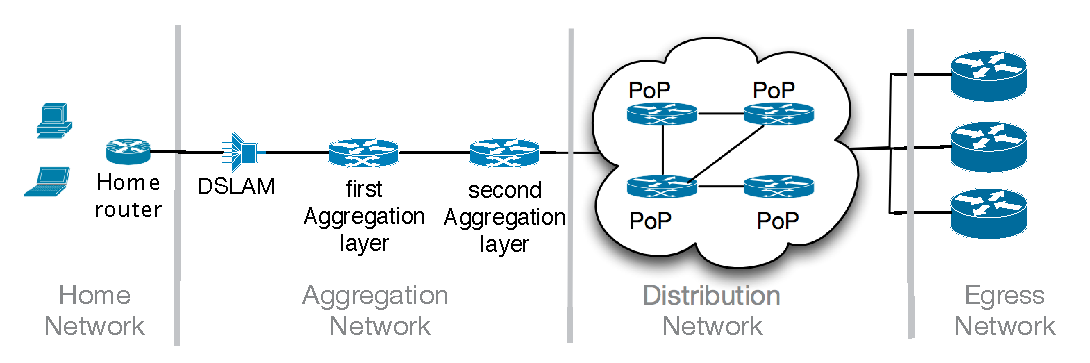
\includegraphics[width=0.95\columnwidth]{isp_plan}
  \caption{\label{fig:isp_plan} The path for each network packet of 
    the home network to the Internet. ISP network can be split in 3 parts:
  The {\it Aggregation Network}, the {\it Distribution Network} and the {\it
    Egress Network}.}
\end{figure}

An equally important problem for existing home networks is the limited ability
of users to control network resource allocation. This problem can be traced back
to two main observations. Firstly, network performance has a multidimensional
definition. Performance requirements may include limits over the  throughput and
latency of a flow and are highly application-specific.  The main approach in
which the ISP address this problem in a fair way between the users of the
network is through the enforcement of monthly or daily traffic
caps~\cite{virgin-caps,bt-caps}.  Rate limiting queues within the network
reduces network utilization, thus reducing packet buffering latencies.
Nonetheless, this approach cannot regulate how network flows share available
resources, as the end-to-end congestion algorithm impacts significantly the flow
resource consumption. Secondly, home network traffic is highly asymmetric.
Upload traffic volumes on average are significantly lower than download volumes.
This is due, in part, to the properties of modern home network links, but also
due to the nature of modern network applications that function in a
client-server manner.  In order to control sufficiently resource allocation a
system should consider independently both directions of the traffic. This
thought is not possible, given the network control limits of the homeowner over
only a fraction of the path. Download traffic, for example, is controlled by the
home owner only on the last section of the path and thus we cannot develop a
sufficient policy enforcing system that has traffic control solely within the
home network limits.

In order to better introduce the reader with our architecture, we present in
Figure~\ref{fig:isp_plan} a simplified depiction of a broadband ISP network.
Although, exact network topologies remain secret, there is a high level design
pattern. In the Figure we present the traversed network devices by a packet send
from the home network to the Internet.  In the Figure, we segment the network
topology in four sections, the {\it home network}, the {\it aggregation
  network}, the {\it distribution network} and the {\it egress network}. The
aggregation network contains the DSLAM that collect the traffic from the user
home over the telephone network, the BRAS that ensures that the received traffic
is in accordance with the ISP policies and a number of layers of aggregation
switches, that multiplex the traffic from the various BRAS on to the
distribution network. Traffic from the aggregation is routed internally within
the ISP over the distribution network in order to reach either to the egress
points of the ISP, or to another aggregation point, if the pattern is destined
to an internal service. The distribution network of an ISP consists of a small
number of large routers with high capacity links. Usually at this point network
administration use network tunnelling tecnhologies, like MPLS, in order to
reduce forwarding information on the routers.  The egress network of the ISP
consist of large routers that are hosted in AS IXP networks and connect the ISP
with peering ASes. 

In the described network design a number of research papers have analysed
latency and bandwidth performance and identified a significant bottleneck in the
last-mile of the network~\cite{Dischinger:2007bg,Akella2003}; the link between
the DSLAM and the aggregation network. The high utilization of this link can be
explained by the high ratio of under-provision of such links. The wide adoption
of broadband access in households has increased significantly resource
requirements and user subscription. Our proposed architecture provides an API
that allows users to exercise flow-level control over the available resources of
the backhaul link.

In the proposed solution we integrate in the ISP network a mechanism that
acquires per-flow information from the users and translates them into
appropriate resource allocations. This approach bridges a fundamental gap
between the views of the ISP and the users. Users perceive network traffic as an
ensemble of flows belonging to a specific application, which applications has a
specific prioritisation in the computer interaction process.  ISPs, on the other
hand, perceive network traffic as an ensemble of network packets aggregated and
operated upon the ingress and egress point within the network. Due to the
homogenous capping policy on packets from the same home, ISPs tend to collapse
any traffic prioritisation of the traffic to or from the home, thus at the
moment reducing the ability of the user to control any resource allocations
enforced at the router level. 

The proposed extension builds around the \of protocol primitive and requires a
switching fabric that can support a rate limiting queue and a prioritisation
based scheduling mechanism for each household. We are aware, from unofficial
discussion with british ISP network administrators, that current ISP networks
have support for similar per-household capabilities in the network. We also need
to point out that we don't consider the proposed solution complete and able to
provide an holistic system to solve the problem of resource scheduling. We only
draw requirement based on observations acquired from relevant user studies and
we are trying to map user demands to relevant network functionality. The
architecture of the proposed system is described in Section~\ref{sec:qos_arch},
while, in Section~\ref{sec:qos_eval}, we present a number of simple experiment
to investigate the behaviour of the proposed system with various types of
competing traffic.

\subsection{User - ISP communication} ~\label{sec:qos_arch}

In the proposed architecture we split the required functionality among three
entities in the network: a data collecting daemon on the end-systems of the home
network, a policy enforcing daemon on the home network router and an
\of-based mechanism to translate user performance requirements to
forwarding policy for the network devices of the ISP.

\paragraph*{End-system}
In order to record the mapping between applications and network flows we have
developed a light cross-platform daemon running on the end-systems of the home
network.  The daemon monitors the connection table of the network stack and
inserts information for each new connection in the HWDB database.  Each inserted
record contains the 5-tuple of the flow and the name of the application that
opened the respective socket.  Mechanisms to intercept new connection events
from the network stack of the kernel are available for most OSes. In our
implementation we use {\it netfilter-conntrack}~\cite{netfilter-conntrack} for
Linux, {\it Windows Filtering Platform}~\cite{win-wfp} for Windows and {\it
  ipfw} for Darwin/MacOSX. These libraries expose similar APIs and allow
applications to register callbacks to the kernel network stack, which are
invoked every time the state of a record on the connection table changes. In
order to match the network tuples with the respective applications, we use the
`{\it lsof}` command in unix-like systems, while for windows we parse the output
of the `{\it netstat -p}` command.

\paragraph*{ISP infrastructure}

\begin{figure}
  \centering
  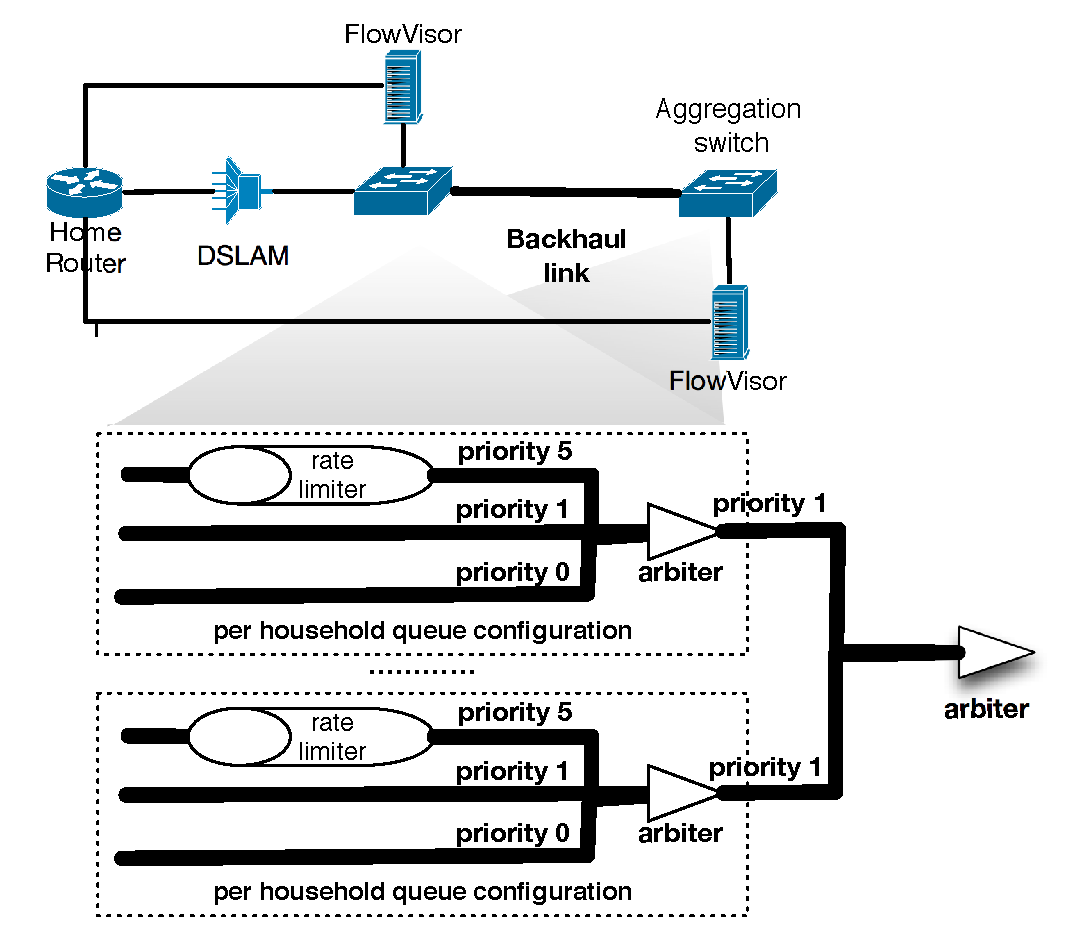
\includegraphics[width=0.8\columnwidth]{queue_design}
  \caption{\label{fig:queue_design} Switches handling the backhaul link expose 
    virtual slices to homeowners through a FlowVisor instance.  Each switch
    configures for each household three queue primitives: A {\it low latency,
      high priority} queue, a {\it medium priority} queue and a {\it default}
    queue}.}
\end{figure}

% In the ISP infrastructure we focus our system on the management of the resources
% on the link that connect the DSLAM with the aggregation layer of the ISP
% network. This link, which is commonly described as the access network backhaul,
% is described in a number of studies as the bottleneck of home Internet
% connectivity. The main reason for being the bottleneck is the fact that this
% point is overscribed, as the bandwith of the link is only a fraction of the
% aggregate maximum bandwidth of the connected homes. 

In order to handle resource allocation on the bottleneck link we propose the
replacement of the switching devices, with \of-enabled switches that support
queue management. The switch control plane is virtualised using the FlowVisor
controller~\cite{flowvisor-osdi}. Each home router is running an \of controller
which connects to the FlowVisor instances on the ISP edge network and exercises
control only over its own traffic. Specifically, the ISP virtualises the \of
forwarding table and exposes only a subset of the entries to each user.
Additionally, each network slice exposed to the homeowners informs the
controller about traffic with a source or a destination IP address equal to the
address of the connection, while flow modification out of this tuple subspace
are discarded by the FlowVisor. This abstraction enforces a strong security
mechanism; home controllers cannot control or evesdrop traffic out of their
scope. 

For each switch and for each home in the network we suggest the creation of
three priority queues: A {\it low latency, high priority}~(LLHP) queue, a {\it
  medium priority}~(MP) queue and a default queue.  The LLHP queue is configured
to have the highest priority from all queues, while it also contains a leaky
bucket mechanism configured to rate limit traffic at a rate equal to the minimum
guaranteed bandwidth of the connection. The HP queue doesn't enforce any rate
limit, but it has a priority which is between the LLHP and the default queue.
By default the forwarding table is initialised with a set of flows to forward
traffic using the default queue. The home \of controller can at run-time modify
the priority of flows, based on the user configured policy.  This capability,
though, is constraint by the number of flows that the FlowVisor exposes to each
home.  The virtualization approach to the ISP network could be further developed
in order to provide a new fairer economical model for the home network; Users
are not charge solely based on the amount of data, but they can enhance their
network performance by purchasing additional flow table entries or higher
guaranteed bandwidth on the edge. 

Because the system in the proposed design exposes a significant portion of the
edge network control to the user, we propose a set of mechanism to nullify the
possibility of a home \of controller to compromise the functionality of the
network.  Firstly, the reduced number of flows exposed to each home ensures fair
utilisation of the forwarding table of the switch. Further, by using the
FlowVisor rate limiting functionality per controller, we can fortify the system
against control plane DoS attacks. Finally, Flowvisor can be configured to
discard flows with an Output action that forwards packet to the incoming port,
in order to restrict the ability of a compromised node to create packet loops. 

\paragraph*{Home Router}

\begin{figure}
  \centering
  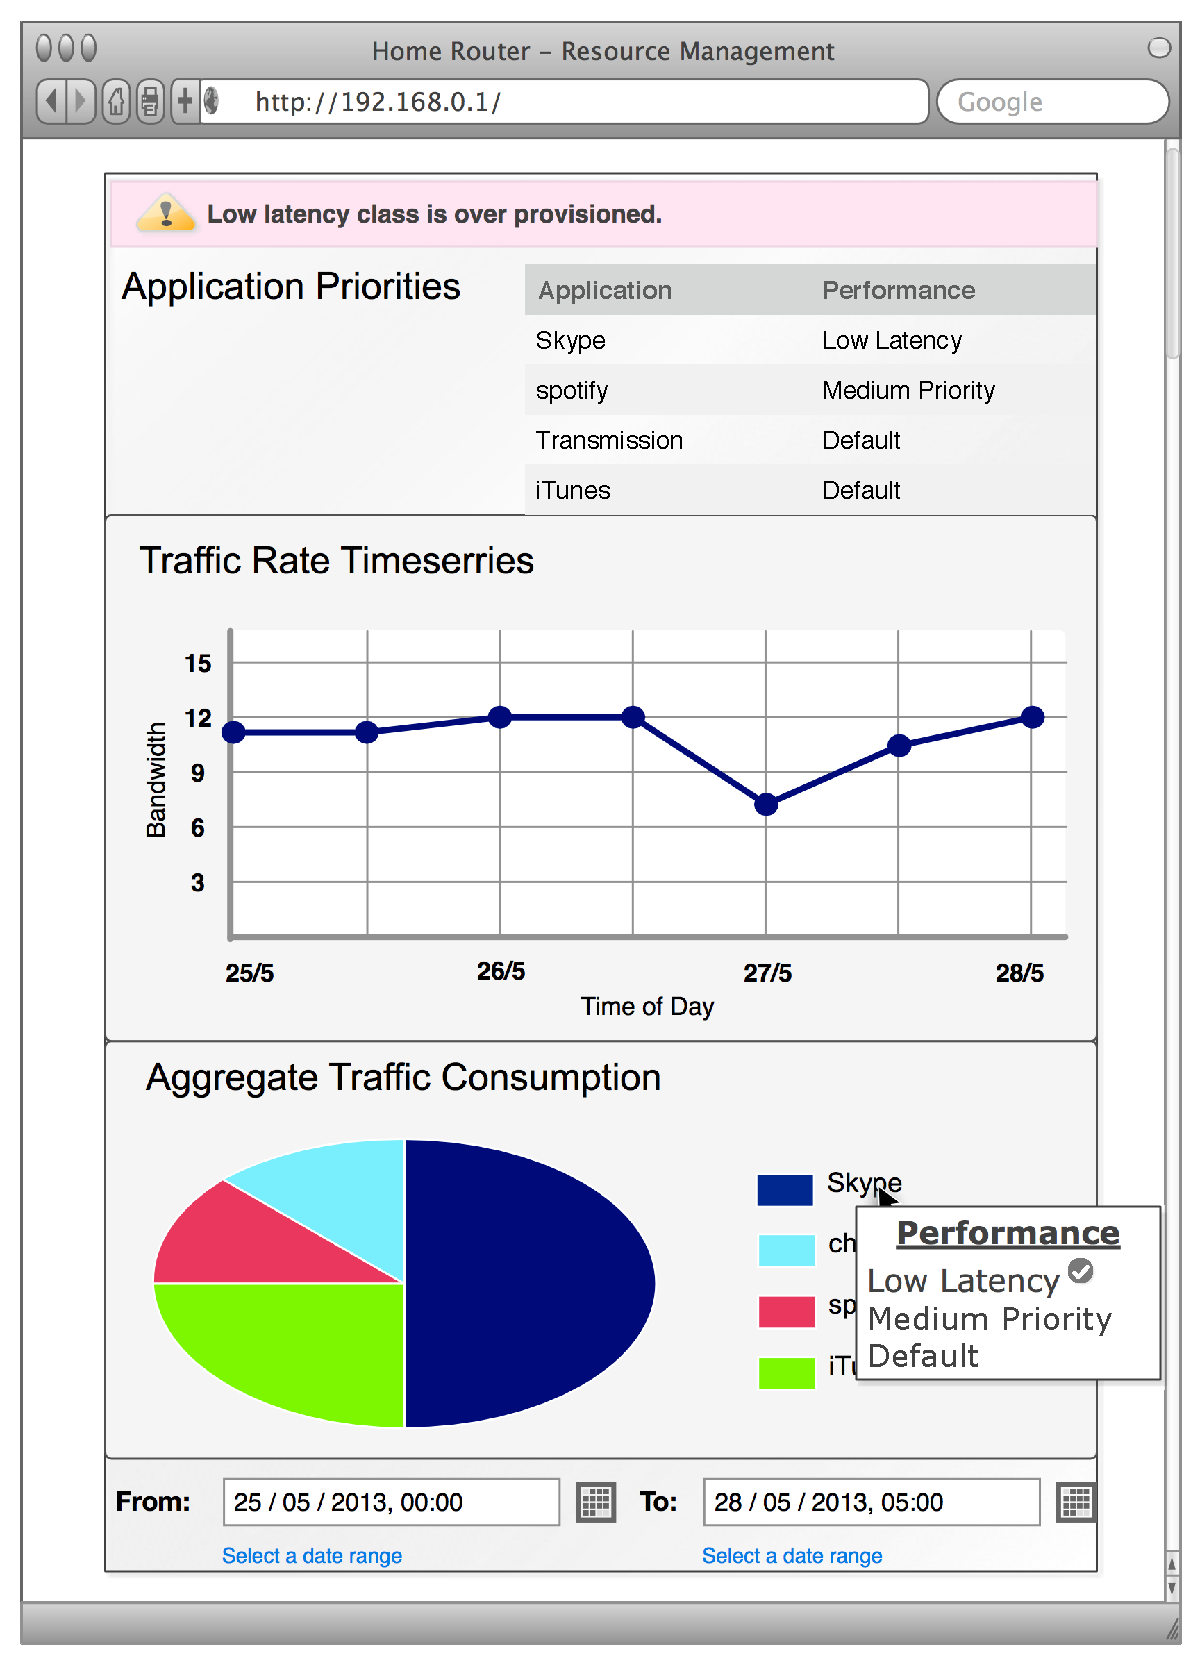
\includegraphics[width=0.8\columnwidth]{homework_intf_qos}
  \caption{\label{fig:homework_intf_qos} Performance mechanism  user control.
    The user is able to view the network utilisation per application, as well as
    express application prioritisation.}
\end{figure}

In our design, we expect the home router to be the rendez-vous point between the
policies of the two network. In order to support the state requirements of this
functionality we add in the hwdb database three new tables: {\it Application
  tuple}, {\it Application timeseries} and {\it Application priorities}.
Application tuple table stores mappings between applications and 
network tuples. This table is populated with data from the end-hosts, while the
router installs a monitoring hook in order to receive new flow arrivals.
Application timeserries table contains timed information on the rate of network
applications. The table is populated with data from the router using the
flow stats message of the \of protocol, while the data are used by the web
visualisation in order to inform users on the network consumption of
applications. Finally, the Application priority table stores the queue mapping
for each application. This table is populated with data from the web interface
of the system while the router uses it to map newly arriving flows to
queues. 

In order to expose in an intuitive way the resource management mechanism, we
design a simple web interface, depicted in Figure~\cite{fig:homework_intf_qos}.
Through this interface the user can be informed on the aggregate resource
consumption of each application, the time serries of the traffic rate per
application and review all priority mappings configured. Additionally, the
interface provides user notifications during incidents of  under-provisioning of
the LLHP queue. Sπecifically, we use the packet loss parameter from the queue
statistics message of the \of protocol and trigger α notification every time
packet losses are detected.  Through this interface we try to address the issues
raised by the work in~\cite{Chetty10}. 

During operation, the proposed design extends the forwarding logic described
earlier. In detail, for each new arriving flow, after the router has verified
that the flow is in accordance with the policy, the
controller will lookup the relevant table in the HWDB and will assign the flow
in the relevant queue, both on the local instance of the OpenVSwitch, as well as
in the remote switches of the ISP. In order to ensure that there is an
application mapping for the flow, in case of an incomming connection the switch
will establish only the incoming direction if the flow on the local switch and
will assign queue only when the outgoing direction of the flow is used. This way
we will have ensured that the end-host daemon will have inserted the appropriate
information. 

\subsection{Evaluation} \label{sec:qos_eval}

\begin{figure}
  \centering
  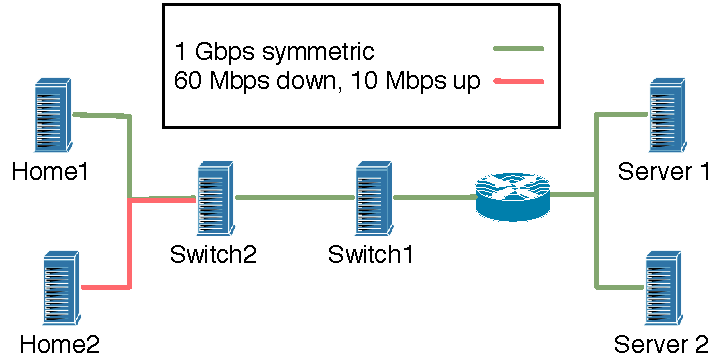
\includegraphics[width=0.8\columnwidth]{queue_eval_setup}
  \caption{\label{fig:queue_eval_setup} Experimental setup to evaluate the
    proposed resource management system.}
\end{figure}


In order to test the functionality of the switch we implemented a lab testbed, 
depicted in Figure~\ref{fig:queue_eval_setup}.

\section{Conclusions} \label{sec:conclusion}

This paper has drawn upon previous user studies to reflect on the distinctive
nature of home networks and the implications for domestic network
infrastructures.  Two particular user needs that arose from these studies were
for richer visibility into and greater control over the home wireless network,
as part of the everyday management of the home by inhabitants.  We  considered
how to exploit the nature of the home network to shape how it is presented and
opened to user control.  

Simply put, the home is different to standard networking environments, and
many of the presumptions made in such networks do not hold.  Specifically,
home networks are smaller in size, the equipment is physically accessible and
access is often shared among inhabitants, and the policies involved are
flexible and often dynamically negotiated.  Exploiting this understanding
allows us to move away from traditional views of network infrastructure, which
must be tolerant of scale, physically distributed, and impose their policies
on users. 

We use the Open vSwitch and NOX platforms to provide flow-based management of
the home network.  As part of this flow-based management, we exploit the
social conventions in the home to manage introduction of devices  to the
network, and their subsequent access to each other and Internet hosted
services.  This required modification of three standard protocols, DHCP, EAPOL
and DNS, albeit in their behaviour only \emph{not} their wire formats, due to
the need to retain compatibility with legacy deployed stacks.
                                                         
Our exploration suggests that, just as with other edge networks, existing
presumptions could usefully be re-examined to see if they still apply in this
context.  \emph{Do we wish to maintain net neutrality in the home?}
Inhabitants do not appear to see network traffic as equal, often desiring
imbalance in performance received by different forms of traffic.  \emph{Must
the end-to-end argument apply?} Householders understand and exploit the
physical nature of their home and use trust boundaries to manage access; we
have exploited these resources to explicitly manage the network.  \emph{Should
communication infrastructures remain separate from the devices that use them?}
In the home setting this separation proves problematic as people, ranging from
the home tinkerer to the DIY expert, wish to interact directly with the
network as they do with other parts of their homes' physical infrastructures.
Our exploration suggests use of a range of displays and devices existing not
as clients exploiting the infrastructure but as extensions of the
infrastructure making it more available and controllable.

Inability to understand and control network infrastructure has made it
difficult for people to understand and live with it in their homes.  We have
developed a home router that both captures information about people's use of
the network and provides a point of interaction to control the network.  Our
initial developments have explored the extent to which residents may be
involved in some of the protocols controlling the network; other protocols
suitable for modification are under consideration.

%\section{Related Work} \label{s:related}
% 
%Many authors have argued that home networks should be treated differently to
%other IP-based networks.  For example, Calvert
%\etal.~\cite{calvert07:_movin_towar_middl} make a case against application of
%the end-to-end principle in home networking.  They argue that there are a
%number of key aspects peculiar to the home environment that the standard
%Internet protocols do not address.  They derive a series of requirements for a
%home network architecture, and a design providing functions to fulfil these
%requirements.  Many of the points they make, e.g., their ``smart middle''
%design, resonate with our argument, and indeed, we believe our home router
%meets the requirements and provides the functions they describe.
%
%%% \mort{no need to spend so much on interfaces- a sweeping ``but they
%%%  don't go deep enough to be interesting'' should be enough}
%Both before and after the general architectural arguments made above, a number
%of authors have proposed novel user interfaces to aid the homeowner in managing
%their network.  GesturePen~\cite{swindells02:_that} uses line-of-sight radio
%interaction with purpose-built receiver tags to control network access;
%Network-in-a-Box~\cite{balfanz04:_networ}, where infrared port alignment
%provides a physical metaphor for access, plugging in to security mechanisms
%such as EAP-TLS and RADIUS.  They also describe an interesting ``phone home''
%service via the Windows Remote Access and IPSec policy mechanisms that enables
%remote clients to connect back to appear as if inside the home network.
%
%ICEBox~\cite{yang07:_icebox} again concentrates on the problem of enabling the
%homeowner to correctly configure new devices when they are brought onto the
%network using a control panel approach similar to our Guest Board.  They note
%that a future version might well subsume the home router.
%Eden~\cite{yang10:_eden}, by several of the same authors, follows this up by
%replacing the home router.  Their implementation allows per-flow traffic
%control, but the paper lacks technical details.
%%   makes use of the standard Linux \emph{tc} and
%% \emph{iptables} facilities to allow the homeowner to exercise per-flow
%% traffic control; they do not discuss technical specifics in any
%% detail.
%
%All these approaches primarily address the interaction design problem, focusing
%on user interface solutions to the problems of managing a home network.  Most
%rely upon specialized hardware or software installation on client devices.  In
%contrast, our home router does not require client modification as its protocol
%modifications are fully backward compatible with existing stacks.  It thus
%supports a very wide range of devices while making possible greater control of
%connectivity.
%
%%% \mort{probably need to leave following refs in}
%
%% Addressing the problems of troubleshooting,
%% Netprints~\cite{aggarwal09:_netpr} is a system for cooperative
%% diagnosis of home network misconfigurations.  They take a black-box
%% approach in that they do not predefine specific models, and they focus
%% on application specific problems rather than the home network as a
%% whole.  Client software scrapes labeled configuration information from
%% devices, and computed feature vectors describing the more dynamic
%% aspects of the system (e.g., observed traffic).  These data are
%% collected in a central server and fed into a decision tree based
%% learning system to perform subsequent diagnoses given observed data.,
%% Kandula \etal.~\cite{kandula09:_detail} also proposed a system for
%% diagnosis of problems, aimed specifically at small enterprise
%% networks.
%
%Several authors have proposed solutions to the specific problem of lack of
%visibility into what the network and connected devices are doing.  In this
%context, HostView~\cite{joumblatt10:_hostv} uses a client daemon to log when
%users experience network problems.
%% also relies on client
%% software but focuses more simply on generating labeled data by
%% enabling the user to notify the system when some user-perceived
%% problem occurred.  
%Calvert \etal.~\cite{calvert10:_instr_home_networ} present requirements for a
%general purpose ``always on'' local logging service, building a simple example
%using \emph{tcpdump} running on a
%NOXBox,\footnote{\url{http://www.noxrepo.org/manual/noxbox.html}} dumping
%traffic into flat files.  Both focus on network monitoring as a tool for
%troubleshooting.  Finally, in presenting the Homework Database, Sventek
%\etal.~\cite{sventek11:_infor_plane_archit_suppor_home_networ_manag} describe
%it as a component in their home network information plane.  Their system uses a
%general-purpose policy engine to exercise control over the network by
%configuration of the router derived from the interaction of monitored data and
%policy.
%
%We claim that, in general, these monitoring systems do not take into account
%the specific challenges and opportunities inherent in the home network context.
%Our home router goes further in exploiting the home context via specific
%modifications to the normal behaviour of key protocols, as well as implementing
%a novel network control interface.
%
%This class of argument, that the generic Internet protocols are not appropriate
%in a particular environment, has previously been made in the enterprise network
%space.  Approaches such as Anemone~\cite{cooke06:_reclaim},
%Ethane~\cite{casado07:_ethan} and Network Exception
%Handlers~\cite{karagiannis08:_networ} have all proposed systems that address
%the general problem of enterprise network management in different ways.  They
%all make the argument that enterprise networks are basically different to the
%traditional Internet, presenting different problems and permitting different
%solutions.  This resonates strongly with our claims that home networks should
%be treated differently, and in some ways with our approach of providing more
%intelligent centralised control.  It should be noted however, that these
%enterprise network solutions are no more applicable to home networks than
%traditional Internet approaches were applicable in the enterprise!
%
%Finally, looking back to 1984 and some of the original discussions of IP
%subnetting, Mogul~\cite{rfc:917} and Postel~\cite{rfc:925} discussed using
%subnetting to hide site LAN interconnection from networks outside the site.
%They introduce techniques such as ARP-based subnetting, ARP bridging, and
%extension of ARP itself.  ARP bridging in particular is very similar in
%practice to the approach we take, although we assign a subnet per-host rather
%than per-LAN, and we manage address allocation and connectivity using protocols
%unavailable at the time.

%% \mort{add intserv, maybe diffserv refs - note different domain and
%%  scale} 

% \section{Conclusions} \label{s:concl}
%  
% This paper has drawn upon previous user studies to reflect on the distinctive
% nature of home networks and the implications for domestic network
% infrastructures.  Two particular user needs that arose from these studies were
% for richer visibility into and greater control over the home wireless network,
% as part of the everyday management of the home by inhabitants.  We  considered
% how to exploit the nature of the home network to shape how it is presented and
% opened to user control.  
% 
% Simply put, the home is different to standard networking environments, and
% many of the presumptions made in such networks do not hold.  Specifically,
% home networks are smaller in size, the equipment is physically accessible and
% access is often shared among inhabitants, and the policies involved are
% flexible and often dynamically negotiated.  Exploiting this understanding
% allows us to move away from traditional views of network infrastructure, which
% must be tolerant of scale, physically distributed, and impose their policies
% on users. 
% 
% We use the Open vSwitch and NOX platforms to provide flow-based management of
% the home network.  As part of this flow-based management, we exploit the
% social conventions in the home to manage introduction of devices  to the
% network, and their subsequent access to each other and Internet hosted
% services.  This required modification of three standard protocols, DHCP, EAPOL
% and DNS, albeit in their behaviour only \emph{not} their wire formats, due to
% the need to retain compatibility with legacy deployed stacks.
%                                                          
% %%                                                          platofrm
%                           
% %% We draw upon these characteristics of the network and the social %%
% conventions of the home to develop two distinct mechanisms, %% implemented
% using the NOX and Open vSwitch platforms as part of a %% redevelopment of the
% home router.  The first exploits the social %% conventions of visiting to
% manage the introduction of machines to the %% network.  This is reflected in a
% modification to the DHCP protocol to %% put people explicitly inside the
% protocol, allowing the homeowner to %% be prompted for advice and information.
% The second exploits the home's %% physical arrangement to develop a physical
% approach to access control %% based on commodity USB storage keys.  
% 
% Our exploration suggests that, just as with other edge networks, existing
% presumptions could usefully be re-examined to see if they still apply in this
% context.  \emph{Do we wish to maintain net neutrality in the home?}
% Inhabitants do not appear to see network traffic as equal, often desiring
% imbalance in performance received by different forms of traffic.  \emph{Must
% the end-to-end argument apply?} Householders understand and exploit the
% physical nature of their home and use trust boundaries to manage access; we
% have exploited these resources to explicitly manage the network.  \emph{Should
% communication infrastructures remain separate from the devices that use them?}
% In the home setting this separation proves problematic as people, ranging from
% the home tinkerer to the DIY expert, wish to interact directly with the
% network as they do with other parts of their homes' physical infrastructures.
% Our exploration suggests use of a range of displays and devices existing not
% as clients exploiting the infrastructure but as extensions of the
% infrastructure making it more available and controllable.
% 
% Inability to understand and control network infrastructure has made it
% difficult for people to understand and live with it in their homes.  We have
% developed a home router that both captures information about people's use of
% the network and provides a point of interaction to control the network.  Our
% initial developments have explored the extent to which residents may be
% involved in some of the protocols controlling the network; other protocols
% suitable for modification are under consideration.  We are currently involved
% in the deployment and study of use of our home router to better understand
% relevant user needs and how we might more systematically exploit the data we
% are collecting.  We are also exploring how to use this data in other areas
% such as security and power management.  


%%% Local Variables: 
%%% mode: latex
%%% TeX-master: "../thesis"
%%% End: 
